
% PAGES: 15
\chapter{Design and Implementation}
\label{mt:c:design}

\section{Analysis of Existing Quadrocopter Architecture}
\label{mt:c:design:Analysis of Existing Quadrocopter Architecture}
Before the focus can be concentrated to the distributed error correction scheme of the \gls{HSE} quadrocopter system, the overall existing architecture has to be introduced in this section. The importance of this introduction causes the necessity to understand and analyse the system which has to be simulated. An overview of the realized and pending components is visualized in figure \ref{fig:ExistingQuadrocopterArchitecture.png}. This overview includes the main systems of the general architecture which are Quadrocopter, Remote Control, \gls{GPS} and the Base Station. Thereby the Quadrocopter is controlled over a permanent unidirectional wireless communication to the remote control, which cyclic sends a pulse-width-sum-signal with the steering information. Thereby the RC-Receiver interfaces a microcontrollers' \gls{ECT} of in the \gls{CCU}, which allows real-time decoding of the information. Further for observing and testing purposes, the architecture allows to observe and to configure parameter and state variables of the quadrocopter in mid-air.
\newpage
To fulfil this, the quadrocopter can send and receive data via a serial\footnote{This wireless communication interfaces the \gls{SCI} of the \gls{CCU}} ZigBee\footnote{See \citebib{Xbee09}} communication to the base station, which runs a Java-Application that captures and visualizes the data and allows configurations in real-time\footnote{Real-time means in this case that the data is pre-buffered at the quadrocopter and asynchronous send to the base station. This allows a fine grained resolution of data capturing and evades time delays of synchronous sending data}. By regarding the quadrocopter system, it can be considered as an architecture with \gls{CCU} mounted and uncoupled components for detecting movements of the system. These components have special behaviour in aspects of resolution, quantisation etc. and bring a impact to the control and flying behaviour of the quadrocopter. 

\begin{figure}[H]
	\centering
		\includegraphics[width=1\textwidth]{graphic/ExistingQuadrocopterArchitecture.png}
	\caption{Existing quadrocopter architecture and future developments}
	\label{fig:ExistingQuadrocopterArchitecture.png}
\end{figure}

\subsection{Central Control Unit}
\label{mt:c:design:Analysis_of_Existing_Quadrocopter_Architecture:Central_Control_Unit}
The \gls{CCU} of the \gls{HSE} Quadrocopter, which is one of the main interesting components in relation with a simulation, is a outcome of a   interdisciplinary corporation of the \gls{HSE} Faculty of Electronics and Mechatronics in G�ppingen 
\footnote{See http://www.hs-esslingen.de/hochschule/fakultaeten/mechatronik-und-elektrotechnik.html} and the \gls{HSE} Faculty of Information Technology Esslingen \footnote{See http://www.hs-esslingen.de/hochschule/fakultaeten/informationstechnik.html}. The dedicated central unit of the \gls{CCU} is a MC9S12XDT256 \footnote{See \citebib[Data-sheet of HCS12X family]{HCS12X07}} microcontroller from Freescale, used for the flight control task.

Additionally the sensors, which are used for the determination of the quadrocopter location in space, are also mounted on the \gls{PCB}. The architecture includes an accelerometer, \footnote{See \citebib[Data-sheet gyroscopes]{LIS05}} that measures the acceleration in \ensuremath{X_B}-, \ensuremath{Y_B}- and \ensuremath{Z_B}-direction, three gyroscopes \footnote{See \citebib[Data-sheet gyroscopes]{ADX07}} for roll-, pitch- and yaw-velocity determination and an air pressure sensor to determine the height. Furthermore a battery sensor (voltage divider) on the board allows the calculation of the new set-points for the brushless controllers 
\footnote{See \citebib[Wiki Brushless Controller Bl-Cl V1.2]{BLCL10}}, because the resulting \glsname{RPM}/thrust of the motors depends on the actual battery voltage.
 For communication with the base station, a XBee \footnote{See \citebib[XBee Pro Module]{XBee09}} module is used directly mounted on the flight control \gls{PCB}. 

Beside that, there are a couple of external interfaces available for remote control, an \gls{IIC} bus to command the brushless controllers and a \gls{BDM} as programming interface. 
\newpage
The interfaces for a distance sensor, a \gls{GPS} receiver and a servo (e.g. for a camera mounting) are available for future extensions (See pending components in figure \ref{fig:ExistingQuadrocopterArchitecture.png})\citeref[p.57 Central Control Unit]{SchSunVetWebFriSat10}.

A closer look on the \gls{IMU}, show that the locations of the sensors are designed \gls{WRT} the velocity or acceleration, which has to be measured. So the sensor which measures the accelerations of the translation movements \gls{WRT} the B-frame is mounted in the middle of the \gls{CCU} to avoid the measuring of rotational components. Similar to that, the gyroscopes also mounted to positions, with the focus to zeroise measurements of unwanted values. So it is possible to describe with these combination of sensors the mathematical model presented in chapter 
\ref{mt:c:literature:s:equations_of_motion}. 
As described in chapter \ref{mt:c:literature:s:Stability_criteria_of_transfer_functions} another important point in digital systems is the quantisation behaviour. In case of the given \gls{CCU} there two aspects which have to be considered. One aspect is the sample time of the control system and the other the resolution, sensitivity, noise etc. of the \gls{IMU}. 

The sample time of the system thereby depends on the load of the microcontroller. This load can be configured or changed  by changing the embedded software with the focus to reduce the load. In contrast to that, the behaviour of the sensors cannot be changed, because these work autarchical and provide the specified performance defined in the data-sheet. 
Based on that, it is important to reflect the behaviour of these sensors in the simulation of the system. As visualised in figure \ref{fig:CCU.png}, the translational sensors provides a different behaviour as the rotational sensors. This causes to the interface and the internal functionality of these sensors. 
\newpage
The acceleration sensor provides a digital readout of the measures via \gls{SPI}. Thereby the quantification is given with the quotient of the gravitational acceleration and the sensor sensitivity
\ensuremath{(g/340)/\glsname{LSb}}  \lbrack \ensuremath{(m/s^2)/bit} \rbrack and the limits, which are specified with \ensuremath{6g} in each direction.

Differently to the digital readout, the gyroscopes which build up the rotational part of the \gls{IMU} provide an analog signal with maximal detection of \ensuremath{5.23 rad/s}, which is represented with a voltage level between ground and reference voltage of 3.3V and need to be digitalized with the controllers' \gls{ADC}. This \gls{ADC} provides a resolution of 10bit and combined with the gyroscope it results to a resolution of \ensuremath{0.0142 (rad/s)/\glsname{LSb}} 
\footnote{The calculations of this chapter are derived from \citebib{CzeSat10}}. So the \gls{IMU} provides measures across the B-frame, 
which fulfil the rotational part of the \gls{GVV} \gls{sym_nu} and the translational part of the derivative \gls{GAV} \gls{sym_dot_nu}.

\begin{figure}[H]
	\centering
		\includegraphics[width=1\textwidth]{graphic/CCU.png}
	\caption{CCU and IMU}
	\label{fig:CCU.png}
\end{figure}

\subsection{Characteristics of Sensors and Actuators}
\label{mt:c:design:Analysis of Existing Quadrocopter Architecture:Characteristics of Sensors and Actuators}
An important aspect in relation to the quality of control, and further the flight behaviour, is the characteristic of the \gls{IMU} and actuators in view of precision. In the case of the \gls{CCU} here, the noise sources are the noise of the \gls{MC}, the noise drift of the 
\gls{MEMS} characteristic in relation to the temperature and the vibration of the motors. Because of this mix of noise sources, the determination of the average noise cannot determined with investigating the data-sheets of the sensors. 

A way of determination, which is executed here, is an experiment which includes the capturing and investigation of the real sensor readout in the preferred hovering state. Experiments with running engines and shut off engines, show that the biggest impact to the total noise originates from the imbalance of the rotors. This effect originates to the fact that small irregularities of the rotors have a big impact to the noise in case of the needed rotor speeds for the hovering state. 

The results of the captured sensor data in a duration of 11 seconds are visualised in \ref{fig:IMU_Analysis_Hovering_State.png} with the corresponding variances \gls{sym_BCSV}, presented in appendix \ref{mt:c:Appendix:s:Characteristics of Sensor Noise}. The \gls{sym_BCSV} in this case is an measure which shows the dimension of noise influence and further the sensor values, which lost because of they cannot detected. 
 
\begin{figure}[H]
	\centering
		\includegraphics[width=1\textwidth]{graphic/IMU_Analysis_Hovering_State.png}
	\caption{IMU noise analysis in the hovering state}
	\label{fig:IMU_Analysis_Hovering_State.png}
\end{figure}
\newpage
The investigation of the actuators can be executed by using a stroboscope with sufficient frequency resolution. This approach also was applied in this project here. The picture \ref{fig:StroboscopeRotorSpeeds.png} visualizes the experiment, which was captured with a satisfactory exposure time of the camera. So the frequency of a rotor can be located, by vary the frequency of the stroboscope. 

Finally the located rotor will optically stand still, and the other rotors will optically rotate in the original direction, or in the reverse direction. This behaviour demonstrates the engines, that run faster or slower as the located engine.

\begin{figure}[H]
	\centering
		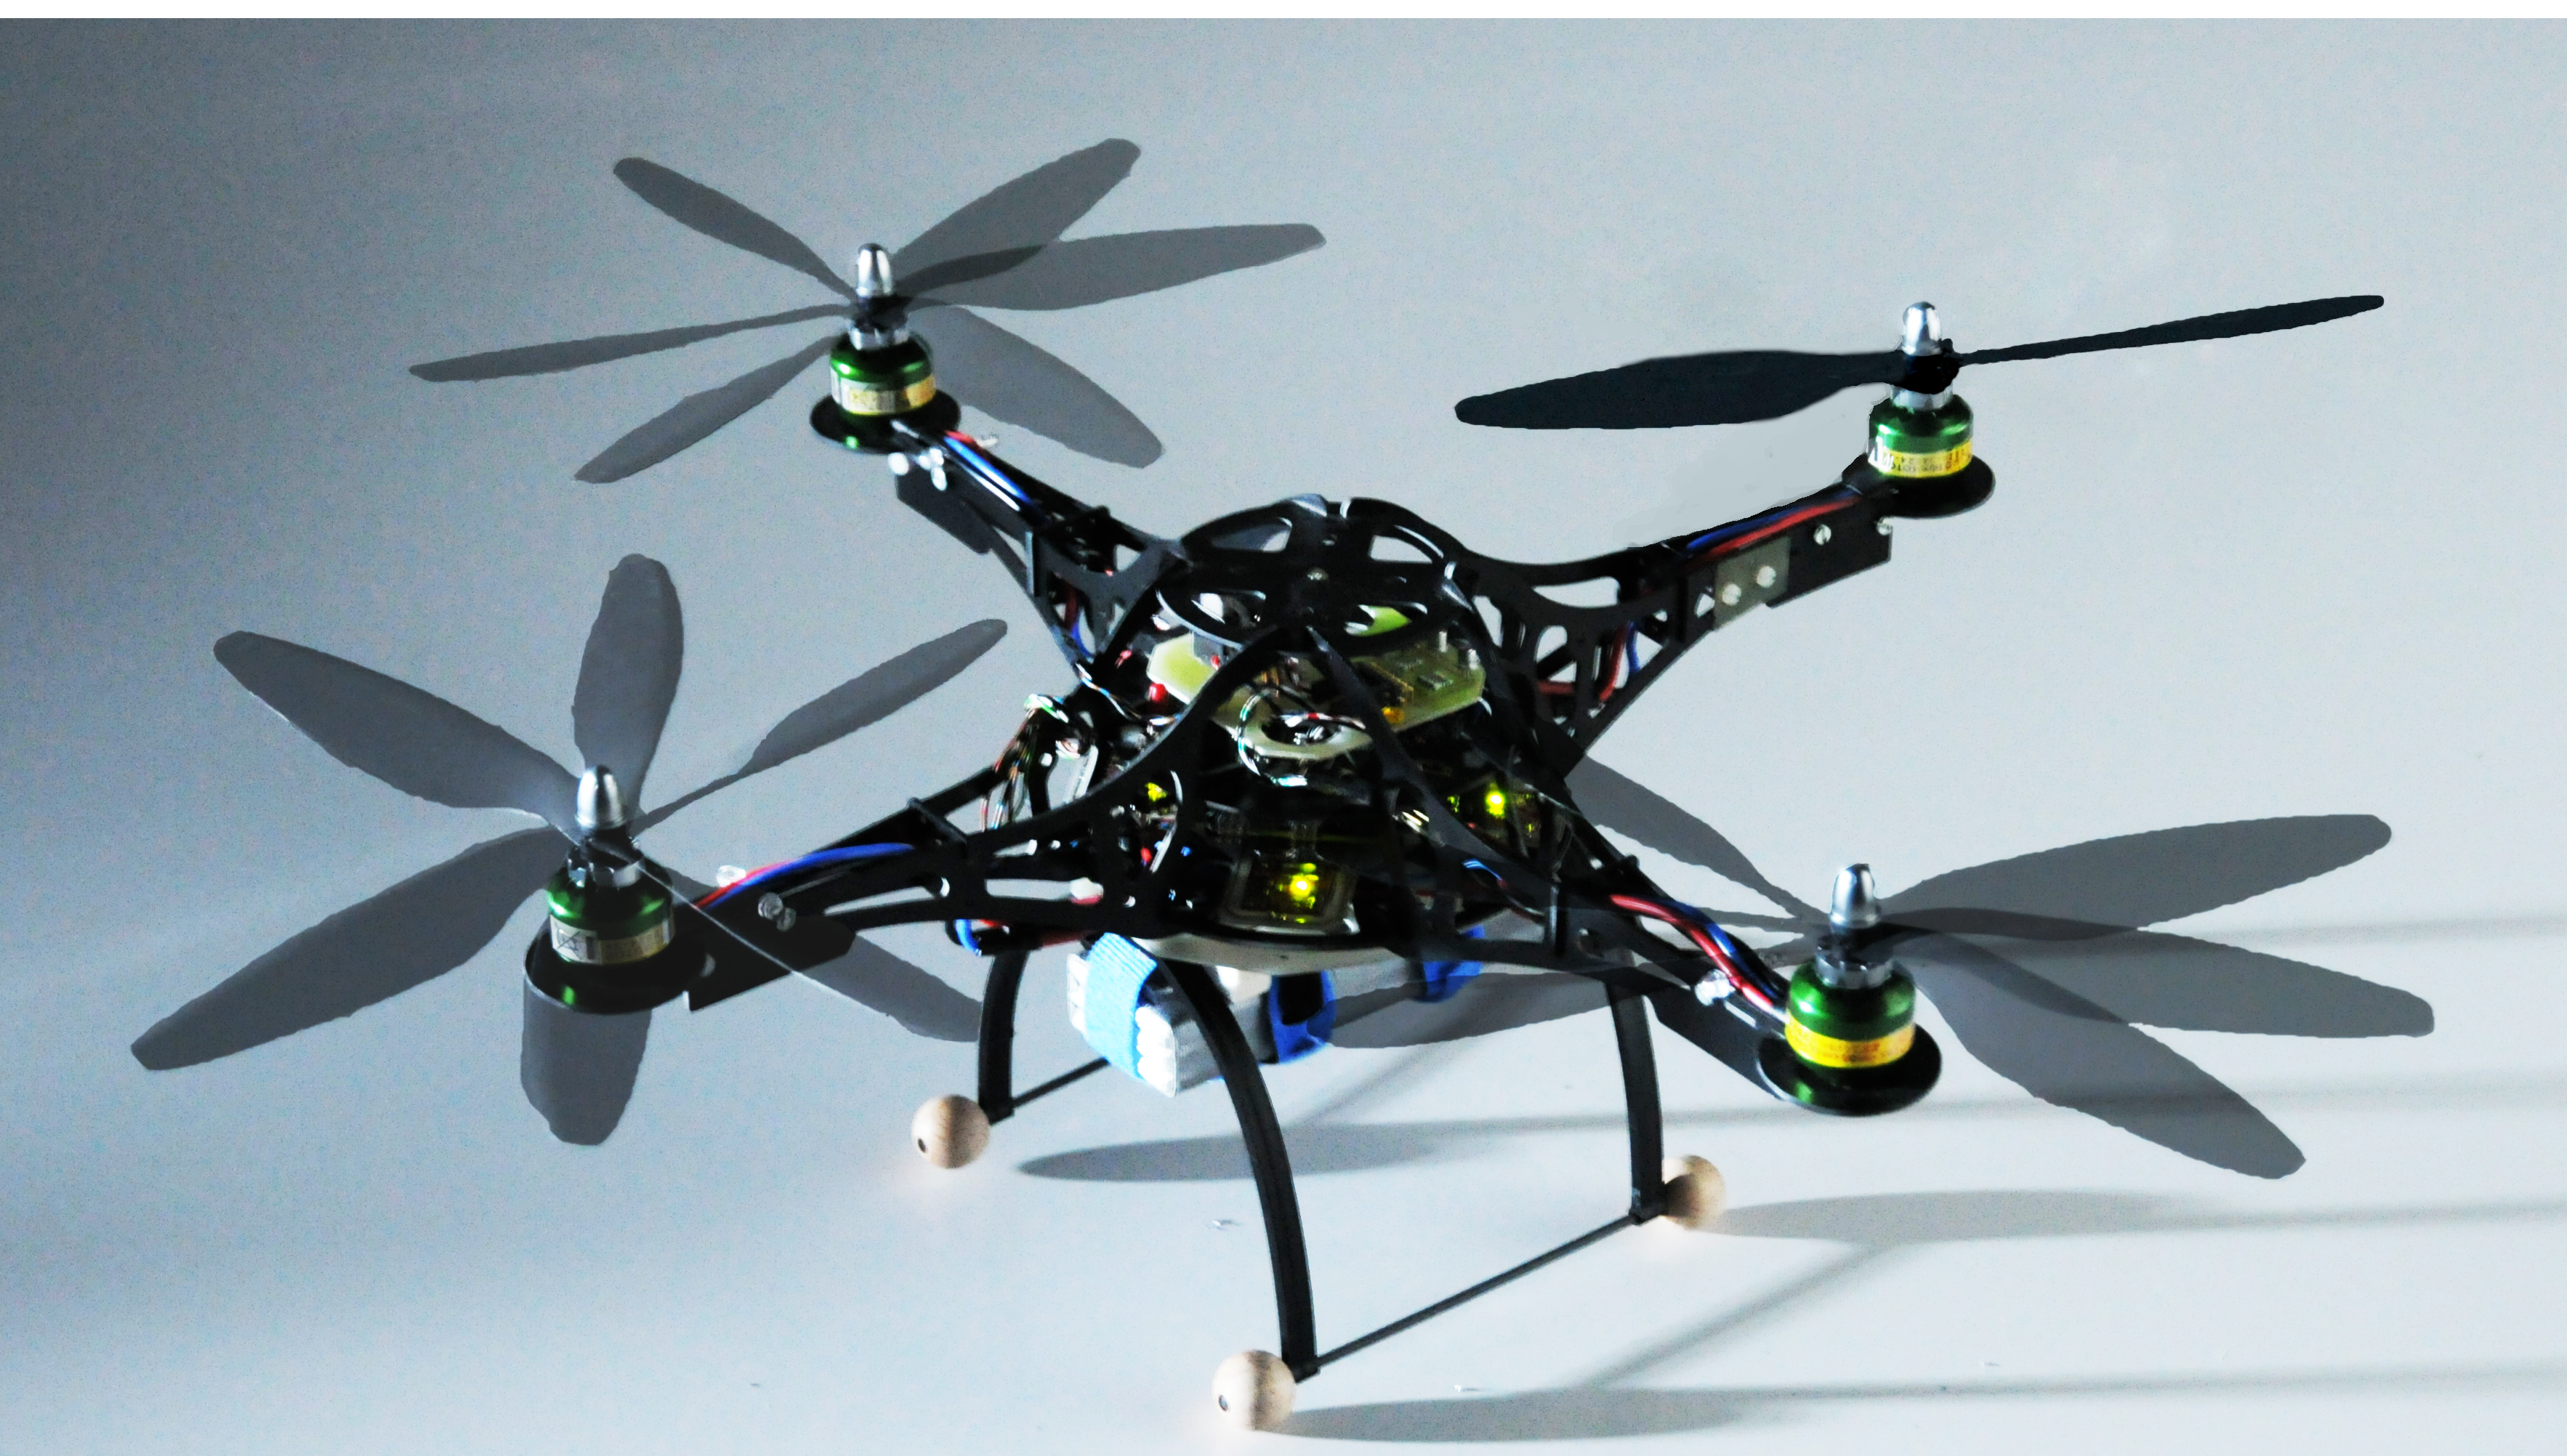
\includegraphics[width=1\textwidth]{graphic/StroboscopeRotorSpeeds.png}
	\caption{Experimental environment for set-point drift measurements}
	\label{fig:StroboscopeRotorSpeeds.png}
\end{figure}

With the execution of the described experiment, it is possible to identify the set-point drift of the particular engines. The results of the 
different set-point drift are visualised in the figure \ref{fig:Engine_Analysis.png}. The mentioned set-point of the engines is a 8bit value, which is written to the control register of the brushless controller. 
\newpage
Thereby the force, that is required to lift up the dead weight of the quadrocopter, is equivalent to the force needed for the hovering state. This force is nearby reached with the set-point of 100 on a scale from 0 to 255. As visualized in the curves in \ref{fig:Engine_Analysis.png}, the particular engines have a characteristic realization of the required set-point input, which can vary from ideal set-point.

These engine characteristics also depend to the mounted rotors and further environmental and physical behaviour which can varies over time. So the exact reconstruction of the engines' characteristics, can be unsuitable for a simulation. A better approach is to define an area different set-point drift are visualised in the figure \ref{fig:Engine_Analysis.png}.

\begin{figure}[H]
	\centering
		\includegraphics[width=1\textwidth]{graphic/Engine_Analysis.png}
	\caption{Set-point analysis of engines}
	\label{fig:Engine_Analysis.png}
\end{figure} 
\newpage
\subsection{Embedded Software Architecture}

Aspects like exchangeability, modular simulation, modular testing and dependency minimisation lead to an encapsulated modular layer design of the embedded software of the quadrocopter. The composition of the quadrocopters' embedded software, shown in the component diagram in \ref{fig:EmdeddedSoftwareArchitecture.png} \footnote{This diagram is derived from the architecture presented in \citeref[p.77 Embedded Software]{SchSunVetWebFriSat10}}, is extended with the real-time behaviour of the call hierarchy. 

Thereby modules, which use an asynchronous interrupt and a corresponding service routine to handle events are marked with a flash icon. Another important information is presented with a special dependency which contains the \gls{CT} of the component call. This value helps to understand and to research the sample behaviour of the sensors and further the control behaviour. Generally as well as in this project here, the \gls{HAL} encapsulates the control registers, which are directly related to the peripherals and the \gls{MC}, and allows a generic access to the functionality of the hardware. 

The quadrocopter \gls{HAL} contains generally five points of service access. These interfaces provide beside the service of initialisation and update of the quadrocopters' real-time image, an access to the communication with the base-station, an on board diagnosis system for noticeable visual and acoustic warnings and the access to the system timer to facilitate \gls{TT} execution in the main routine.
\newpage
Further the real-time image, located in the data layer, provides a protected access to the actual state and data of the quadrocopter. So the state of the quadrocopter is accessed by the application layer uncoupled from the \gls{HAL} and at a central data pool which allow only one state of each value. At the top level of the layer architecture, the application layer contain the control, filter and base-station communication logic of the system. Thereby the main routine uses a \gls{TT} call strategy to realise \gls{DMS} with specific \gls{CT} of the components. 

Two important points of this scheduling architecture, also described by Audsley et. al \citebib{AudBurRicWel01}, are the fact that the sum of the execution times of every routine (including \gls{ISR}) has to be smaller as the smallest deadline, which is in this case 5ms, and further the biggest deadline has to be smaller as the repeating period of execution. This constraints limit the calculation complexity of filter, control or further on-Board algorithms drastically and have to be considered in further developments and simulations.

\begin{figure}[H]
	\centering
		\includegraphics[width=1\textwidth, height=1\textwidth]{graphic/EmdeddedSoftwareArchitecture.png}
	\caption{Software components and their relationship of the Embedded System Quadrocopter}
	\label{fig:EmdeddedSoftwareArchitecture.png}
\end{figure}


\section{Adopted Approach}
\label{mt:c:DesignAndImplemetation:Adopted_approach}
After the introduction of the existing quadrocopter architecture and the analysis about the relevant characteristics of the soft- and hardware-modules, the adopted approach which will researched here is presented in this chapter. 
\newpage
Based on the introduction of the distribution approaches, presented in chapter \ref{mt:c:LiteratureReview:Distribution and implementation approaches}, the \gls{ONCA} in combination with \gls{OFIP} and \gls{SWBIP} approach will be researched here. As mentioned in the comparison of these approaches, the advantages and disadvantages are related to the aspects of interesting. So the aspects of simulation prototyping and behaviour investigation of the image processing, as well as the delay tolerances in relation to the control behaviour lead to the mentioned approach decision. As shown in figure 
\ref{fig:AdoptedApproachArchitecture.png} the adopted architecture is composed of the simulation of the base station with the corresponding image processing and the simulation of the quadrocopter components which are in focus of interest. Beginning with the set values of the embedded system, the remote control component provides time variant signals of the angular set values for roll and pitch, the angular velocity value of yaw \gls{WRT} the B-frame and the thrust value. These set values are the primary input for the body related control, which interfaces the physical model simulation with the same input values, which are provided from the \gls{CCU} and the output values. Withal the input values are transformed to a desired form, which is used for \gls{PID} control. Beside the \gls{IMU} values of the \gls{CCU}, the physical model provides an image sequence related to the position values of the quadrocopter \gls{WRT} the B-frame. Thereby the image capturing process is simulated with a high resolution underground image and the projection of the desired image resolution on it. These image sequence is provided to the simulated on-board vision system according to the \gls{ONCA} architecture. Further the vision system includes a  send process with an output image-buffer to provide the images to the base-station, and an receive process with an input correction-value-buffer.
At the other side of this wireless correspondence the base-stations' process also uses a buffered \gls{I_O}, and determines the translation (u and v) and rotational values (\gls{sym_r_of}) from the calculated \gls{OF} field.
\newpage
Finally the additional controller, which realises the drift elimination in the hovering state, is located in the quadrocopter system and observes the set values of the remote control. The idea thereby is to find a value state of the set and sensor values, which symbolises that the hovering state is desired by the pilot and further the quadrocopter body is ready to reach that state. To realise that behaviour a state machine, which is located in the module "Check Hovering State", decides in real-time the activation of the visual system. So the set values of a second controller, that is located in the separate position control module, are switched from zero to the received correction values. This has the effect that the body controller is delegated by the second position controller and corrects the position with a correction flight manoeuvre. If the pilot sends new set values, after the quadrocopter has reached the hovering state, the position controller is deactivated and allows the pilot and further the body controller an uninterrupted flight and batch-processing of set values. 
% Why state machine observes just set values?
% Description of Distributed error correction scheme

\begin{figure}[H]
	\centering
		\includegraphics[width=1\textwidth]{graphic/AdoptedApproachArchitecture.png}
	\caption{Adopted approaches' architecture}
	\label{fig:AdoptedApproachArchitecture.png}
\end{figure}

%\subsection{Optical Flow Approach}
%Short overview of approaches Ref to chapter 3.2.4. Why block matching -> fundamental approach, less parameters to configure.
%Describe the Optical Flow interpretation
%Generally two of the classifications of \gls{OF} algorithms are given with algorithms which uses a feature tracker and algorithms which search pixel groups, called blocks, between the sequence of images. The feature tracker algorithms first determine good trackable features. This features used as base, and searched in the following sequence of images. The vectors, calculated between these sequence of features, result the \gls{OF} field. In this project here, this kind of \gls{OF} determination is used with a corner detection process as feature tracker. In the other hand, a block matching algorithm is used to fulfil a comparison of two algorithms of different classifications. Beside the specific algorithm of the \gls{OF} determination, the calculation and processing of the vector field also represents an important topic of investigation. The approaches used here are visualised ...

\subsection{Control Approach}
\label{mt:c:DesignAndImplemetation:Adopted_approach:Control_Approach}
Before starting the design of the quadrocopter controller, it is helpful to understand and analyse the abstract behaviour of the separated, physical processes and to proof the correct function of the approach. This strategy lead in this project here to the construction of a simulation which shows the behaviour of realising an angular set-point value to one axis of the quadrocopter, which include two engines as actuators. As visualised in figure \ref{fig:QuadrocopterPhysicalModel}, two opposing engines realise the angle movements in the specific pitch- or roll-axis. These engines can realise an individual gain to the given set-point and influence the precision of the control system. Another point which is problematically in this case is the fact that the feedback angle acceleration of the \gls{CLCS}, has to be integrated two times. 

The combination of the unprecise gain of the engines and the two integrations influences the stability of the \gls{CLCS} enormous. To simulate this behaviour and to impart the expected effects, a abstract simulation is build up and executed in Simulink with two configurations. As visualised in \ref{fig:PIDCascadeCtrl.png} the plant includes two engines, simulated as a sequence of a direction and individual gain. Furthermore two integrators transform the angular acceleration to a angular velocity and position which is used for feedback for the cascaded \gls{PID}-Controllers. This feedback is designed as switch which can be interrupted, to fulfil a tests scenarios with single and cascaded 
\gls{PID} control approaches.

\begin{figure}[H]
	\centering
		\includegraphics[width=1\textwidth]{graphic/PIDCascadeCtrl.png}
	\caption{Abstract CLCS of one angle}
	\label{fig:PIDCascadeCtrl.png}
\end{figure}

As introduced in chapter \ref{mt:c:literature:s:Control_Systems_Characteristics}, the stability behaviour of \gls{CLCS} can be shown with a pole diagram and the investigation of the location of the poles (See Pole Map \ref{fig:PIDCascadeDiagrams.png}). Another method, to proof the stability in the frequency domain, is given with the Nyquist Criterion \citeref[pp. 487-493, Relative stability and Nyquist Criterion]{DorBis01} and describes that each integration in a system affect a shift of \ensuremath{90�} of the frequency phase. The criterion describes that the phase at the x-axis' point of 0dB of the corresponding gain has to be bigger as \ensuremath{-180�}. So also this theorem proofs, that the determination of a value which passes two integrators, must have a \gls{PID}-cascade to ensure that the feedback prevents a critical frequency phase shift.

These relations are visualised as bode diagram in figure \ref{fig:PIDCascadeDiagrams.png} with logarithmic axis of the gain, frequency and phase. Furthermore the step response of the \gls{PID}-cascade and the single feedback \gls{PID}-controller (See Step Response \ref{fig:PIDCascadeDiagrams.png}) shows the stable and the oscillating unstable behaviour of these configurations.

 
\begin{figure}[H]
\subfigure{\includegraphics[width=0.33\textwidth]{graphic/PIDCascadeDiagrams_1.png}}%\hfill
\subfigure{\includegraphics[width=0.33\textwidth]{graphic/PIDCascadeDiagrams_2.png}}
\subfigure{\includegraphics[width=0.33\textwidth]{graphic/PIDCascadeDiagrams_3.png}}
	\caption{Pole Diagram, Bode Diagram and Step Response of one angle system}
	\label{fig:PIDCascadeDiagrams.png}
\end{figure}


\subsection{Problems, Limitations and Assumptions}
\label{mt:c:DesignAndImplemetation:Problems_Limitations_and_Assumptions}
This chapter focus the existing problems in the real implementation of a distributed, visual drift correction scheme
of \gls{UAV}, and shows abstractions and assumptions that are made for the structure and implementation of this projects' simulation.
Such characteristics can be separated into domains, which provide the basis of problem and limitation analysis and allow to define a
abstraction level. This abstraction level can be used to focus and analyse, just the characteristics of a specific part of a solution. This allows to concretise and locate problematic behaviour before searching for a solution at a wrong section. A concrete example for this argumentation can be given by regarding the camera domain. 

Characteristics like the focal length influences the sharpness of the image and influences the 
image processing algorithm to calculate the \gls{OF}. But this characteristic can be classified as problem, that has to be solved after the characteristics of more basic problems has been investigated. 
\newpage
The focal length f can be abstracted with setting the height Z, between the image plane of an ideal projection model and the underground, equal to f and to assign both values the fixed value of one meter. This allows to project the values of the ground points \ensuremath{P=(X, Y, 1)^{T}} directly to points on the image plane \ensuremath{p=(x, y, 1)^{T}} 
\footnote{A detailed mathematical deviation of this abstraction presented in \citeref[Chapter 2, pp.15-16 instructions of transformation]{Fac08}}. Further assumptions of the camera domain are, the camera does not create distortions 
\footnote{This fact also is implicated with the usage of the ideal projection model}, the optical axis is projected rectangular to the underground \footnote{This implicates that the camera movement is planar to the ground and the camera is mounted correctly on the \gls{UAV}. This assumption is adopted from \citeref[p.78 Motion Model Deduction]{Wei09}} and the exposure of the environment is constant over time
\footnote{Experiments with a real camera involve a correct camera calibration (see appendix 
\ref{mt:c:Appendix:Mathematical_description_of_distortions}), and a environment preparation of the exposure to realise these characteristics}.
So the assumption in relation of the \gls{DOF} of the camera system can be described as same as the \gls{DOF} of the quadrocopter body, but reduced in the rotational movements around the axis which originates in the middle of the image plane. The quadrocopter body domain defines the behaviour of the movements of the hovering state, which can be assumed as a 5 \gls{DOF} by reducing the movements across the axis \ensuremath{Z_B}. The realization of these two different \gls{DOF} system can be realized with a real-time image correction process as described in 
\ref{mt:c:Appendix:Mathematical_description_of_distortions} or with a hinge mechanism which keeps the image plane planar to the ground. 

In the simulation this assumed state of the camera domain is realised with a state machine and the orthogonal projection of a simulated camera image on a underground image, as mentioned in chapter \ref{mt:c:DesignAndImplemetation:Adopted_approach}. Another domain, which includes limitations and has to be defined here, is given with the underground domain. The related assumptions to this domain, are that no objects exist, which moving relative to the quadrocopter e.g. no moving light reflections, and the underground image contains points and contrast,
\newpage
which can be evaluated in the \gls{OF} algorithm. For example, an underground image of a snow-covered landscape which contains segments with no contrast is not usable for this approach. Finally the communication between the base-station and the quadrocopter is abstracted as delay. This abstraction excludes communication fail, synchronisation or segmentation problems and assumes a smooth operation of the image and correction value transmission and reception. This behaviour is also symbolised with synchronous buffering systems in figure \ref{fig:AdoptedApproachArchitecture.png}.

\begin{figure}[H]
	\centering
		\includegraphics[width=1\textwidth]{graphic/ProblemAndLimitationDomains.png}
	\caption{Problems and limitations separated in domains}
	\label{fig:ProblemAndLimitationDomains.png}
\end{figure}

% Description of abstractions and assumptions
% Starting Problem of image processing
% Angle of the camera
% Distortions
% Light effects
% Noise
% Problem of relative moving Objects -> Background estimation
% Problem of captured underground -> Snow no features? etc.
% Directory Problem of yaw causes sign of vector
% Aperture Problem

%Assumption 1 Vehicle moves on a planar ground plane. This assumption is true
%for vehicle under most circumstances and it limits the degrees of freedom of the vehicle
%moving on this plane. [Wei09, S.74]
% How I guarantee this in the implementation? -> State Machine
%
%Assumption 3 The XZ plane of the camera frame is parallel to the ground plane.
%This assumption is valid if the camera is mounted on the vehicle correctly.  [Wei09, S.78]
% How How can I simulate such thing? -> Image Projection on large image 

%Assumption 4. Communication is abstracted as delay, no errors no copies no synchronisation
%problems, etc.
%Der Kommentierte Text wurde in diesem Kapitel eingebaut

\section{Simulation of Embedded System Quadrocopter}
\label{mt:c:design:Simulation of Embedded System Quadrocopter}
The architecture of the embedded system simulation is constructed by following the modular design.
\newpage
The focus of this execution was to full-fill the aim of an exchangeable and flexible simulation architecture, which can be changed and reconfigured with minimal effort. This design criteria results to the architecture of Simulink modules as visualised in \ref{fig:SimEmbSysQuadro.png}, and allows a hierarchical realisation of the quadrocopters' system simulation. The separation of modules contains a control library which allows to use several control modules in relation to the development state.
As shown, the first development is executed as prototype in a native Simulink model without having complexity or resource limitations. This model is refined to an embedded \gls{MATLAB} model, which contains only Matlab code which is cyclic executed. This refinement allows to simulate the quantisation and limitation behaviour of an embedded controller and further to evaluate if the implementation algorithm works correctly. The last step is to implement or to generate the embedded controller to the quadrocopters' embedded system target language C, and to evaluate this with the \gls{HIL} module over a serial interface. This last step includes aspects like resource limitation analysis, algorithmic calculation complexity etc. 

Based on this method, this project here focus the development of a Simulink controller in the abstract level by using the \gls{IMU} and \gls{OC}, which can be implemented and realised in the same way as the existing control algorithm which controls only by using the \gls{IMU}. The sensors and actuators are grouped in a own library and allow generic customisation of a sensor and actuator model and can be exchanged if the real hardware is changed. This exchange behaviour is also given in other components of the embedded quadrocopter system simulation and can be extended with implementation of new modules \gls{WRT} the interface architecture.
\newpage
The optical-sensor has a special function in this project. It allows running tests and simulations of the quadrocopter system with a reduced simulation complexity. This is fulfilled because this module can generate the behaviour of the image processing signal with mathematical functions and can so reduce the simulations' execution time. Finally the utility library contains tools for analysis, visualisation and steering of the quadrocopter simulation, which have an important function in the performance test process of this project.  

\begin{figure}[H]
	\centering
		\includegraphics[width=1\textwidth, height=1\textwidth]{graphic/SimEmbSysQuadro.png}
	\caption{Modular overview of the Embedded Quadrocopter System Simulation}
	\label{fig:SimEmbSysQuadro.png}
\end{figure}

The customised embedded quadrocopter system architecture is shown in figure \ref{fig:CustomEmbSysQuadro.png} as Simulink model, which contains a \gls{CLCS} architecture. The set-values from the remote control can be generated in different ways and support a virtual flight with a 3D-mouse or further a flight manoeuvre constellation of steering values. This signal is a composition of pulses defined with the Heaviside-function \footnote{See \citebib{Wei11}} and multiplied with ramp-signals and can be accessed for batch-simulation. 

These set values are realized in motor values by the control component. This component executes, with respect to the mentioned development state, a controller simulation till a \gls{HIL} communication. In each case the controller knowledge of the quadrocopter movements are provided by the sensors. In this special customisation the input signals of the sensors are provided by the Dynamics block and can be assumed as optimal. 

Thereby the sensor block provides the signal with disturbances like noise and quantisation as in reality. Further the correction values for the drift elimination are already known by the  sensor block and can be also disturbed by regarding the signal quality of the optical movement detection. Another way to determine these correction values is to send these via the output of this model to the base station and to receive the corresponding correction.

The signal pos-vel-acc includes all signals, produced by the Dynamics block, and provides a generic interface between the related collaborative blocks. Another strategy to test the stability of the control algorithm is the generation of environmental influences. This can be executed  similar to the remote control with the generation of a velocity vector signal stimuli, which is add as error to the actual optimal velocity value calculated by the \gls{EOM}. 
\newpage
To provide the opportunity of batch-processing-simulation, the error signals can also be accessed outside the model. 


\begin{figure}[H]
	\centering
		\includegraphics[width=1\textwidth]{graphic/CustomEmbSysQuadro.png}
	\caption{The customised CLCS architecture in Simulink}
	\label{fig:CustomEmbSysQuadro.png}
\end{figure}

\subsection{Flight Dynamics}
% Realizations of Flight Dynamics -> Inputs and Outputs errors
% Results from the Thrust to Seitpoint Curves in chapter 4.1.2
%% Further characteristics of motors
% Input transformation process output?
\label{mt:c:DesignAndImplemetation:Flight_dynamics}
The realisation of the dynamics block in Simulink is based on the researches presented in chapter 
\ref{mt:c:design:Analysis of Existing Quadrocopter Architecture:Characteristics of Sensors and Actuators} and on the 
\gls{EOM} presented in chapter 
\ref{mt:c:literature:s:equations_of_motion}. First the derived \gls{GAV} \gls{sym_dot_zeta} \gls{WRT} the H-frame was analysed to determine the dependencies of the \gls{ODE}. Based on that, the physical model was build up  with the aim to ascertain all positions, velocities and accelerations of the quadrocopter body, that is required for this project. The result is presented in a schematic view in the figure 
\ref{fig:SimulinkImplementationOfDynamics.png}. Thereby this module gets the register set-values, corresponding to the brushless controllers in the reality (See\ref{mt:c:design:Analysis of Existing Quadrocopter Architecture:Characteristics of Sensors and Actuators}), and passes the mentioned pos-vel-acc vector to the next block.
\newpage 
In this process the actuators engine blocks transform the set-point to a corresponding force \ensuremath{F_n} \footnote{The index n stands for the number of engine and ranges from 1 to 4} and \gls{RPM} value \ensuremath{\Omega_n} (See \ref{mt:c:DesignAndImplemetation:Sensors_and_Actuators}). 

These values of the different motors are composed to the movements \ensuremath{U_n}, by executing the calculations presented in equation \ref{formula:EB_Omega2} and further to the resulting \gls{RPM} value \ensuremath{\Omega}. Furthermore, these output values are passed to the calculations, which based on the component \gls{sym_dot_omega_B} \gls{WRT} the B-frame of the equation \ref{formula:dot_zeta}. To determine the velocity and the angle, this vector is integrated two times. A special behaviour of this block is that the calculation of the \gls{sym_dot_omega_B} needs also its own values. So the start values have to be initialised in this case for the initial execution with the values zero. Equivalent to the B-frame component of \gls{sym_dot_zeta}, the E-frame component \gls{sym_ddot_Gamma_E} from the equation \ref{formula:dot_zeta} is used to calculate the translation acceleration, velocity and position vectors. Thereby the translations also passed trough two integration processes. 

\begin{figure}[H]
	\centering
		\includegraphics[width=1\textwidth]{graphic/SimulinkImplementationOfDynamics.png}
	\caption{Schematic realisation of Dynamics Module }
	\label{fig:SimulinkImplementationOfDynamics.png}
\end{figure}

These calculated values are combined to the output vector and provided as output. The \gls{GVV} \gls{sym_V_B}, which is needed to simulate the on-board behaviour of the acceleration sensor, is determined with the inverse rotational matrix multiplied with translation \gls{GVV} \gls{sym_Gamma_E}. The generic aspect of this approach is that a generally \gls{EOM} dynamics model also will have the same output values and will be compatible to the same interface, if it has 6 or less \gls{DOF}. Furthermore the determination of all movement values allows the simulation of future developments with each kind of movement detection sensor.

\subsection{Control}
% Realization of control approach -> Inputs, Outputs Design Cascade
Observing the analysed control behaviour, presented in chapter \ref{mt:c:DesignAndImplemetation:Adopted_approach:Control_Approach}, the final quadrocopter controller is a \gls{MIMO} controller, which includes several cascaded \gls{PID} \gls{SISO} controllers. The figure 
\ref{fig:QuadrocopterControlArchitecture.png} visualises the detailed controller architecture. Starting at the input values of the control module the angular velocities, the translational acceleration values and the set values are combined for control usage. Thereby the different sources of the values are symbolised with superscript symbols like "Gyr" for gyroscope, "Opt" for optical sensor, "Acc" for acceleration sensor and "Set" for set-value. These input values run first through a process of transformation, which converts the raw sensor values to usable physical values for the control process. In this case the angles for pitch and roll are not determined with an integration but are calculated using the translational accelerations of the corresponding rotation axis. 
\newpage
This is possible because the gravitational orthogonal force is related to these rotations and can be used to determine the angles without an integration process. The conversion of raw- to physical-values, presented in chapter \ref{mt:c:design:Analysis_of_Existing_Quadrocopter_Architecture:Central_Control_Unit}, allows an easier control realisation and processing. 

\begin{figure}[H]
	\centering
		\includegraphics[width=1\textwidth]{graphic/QuadrocopterControlArchitecture.png}
	\caption{Quadrocopter Control Architecture}
	\label{fig:QuadrocopterControlArchitecture.png}
\end{figure}

The converted physical values are passed to the position-correction and body-control-process. Thereby the position-correction-process passes the set-values to an internal state-machine which detects the hovering state and activates the position-correction-controllers. For realising this, the state-machine checks the set-values of the angles and checks if these are smaller as a defined threshold, which symbolises that there is no activity of the remote control. After reaching this threshold the state-machine switches to a state which delays the activation of the position-correction-controller for the duration of \ensuremath{t_{wait}}. 
\newpage
This delay is needed for the body controller and the related cascaded \gls{PID} controllers to reach the steady-state of the hovering position. The activation of the position-controllers, which try to minimise the input values of the optical sensor, affects that the output values of these controllers are integrated to the first stage of the cascaded \gls{PID} controller in the body control. The result is that this collaboration of the controllers affect the needed behaviour for position correction of the hovering state, because the error value of one controller architecture is passed as set-value to the other architecture. Finally the cascaded \gls{PID} control realises movements given from remote control, or manoeuvres needed for position correction, and passes the angular values to a conversion block for the motor set-points. This block realises the variations of the particular motors by realising the desired thrust set-value \ensuremath{U_1}. Another important characteristic in the design of this simulation is the option to run the body and position-control \gls{PID} controllers with different sample times (\ensuremath{t_{s}^{opt}} and \ensuremath{t_{s}^{imu}}). This behaviour originates form the facts, that the \gls{IMU} sensors can provide a higher sample rate as the optical sensor, and the sample rate can influence the characteristics of a \gls{CLCS} (See \ref{mt:c:literature:s:Stability_criteria_of_transfer_functions}).



\subsection{Sensors and Actuators}
\label{mt:c:DesignAndImplemetation:Sensors_and_Actuators}
A simulated dynamic model, as introduced in chapter \ref{mt:c:DesignAndImplemetation:Flight_dynamics}, provides as mentioned optimal movement  signals, which does not reflect the reality. So an artificial process which creates a disturbing signal fused with the optimal signal, can be used to investigate and simulate the realistic behaviour of the sensors and actuators. These characteristics are also regarded in this project here with the result to transform the optimal signals with the experienced knowledge of chapter \ref{mt:c:design:Analysis of Existing Quadrocopter Architecture:Characteristics of Sensors and Actuators}.
\newpage
The results are presented as Simulink models in \ref{fig:SensorsAndActuators.png}. 
Both components, sensor and actuator, contain similar functions to limit and amplify (Saturation and Gain) the incoming signal. Gyroscope and acceleration-Sensors further contain a quantification, offset and noise process to fulfil these typical effects. The sensor model can so be customised individually by configuring these mentioned characteristics, and provides a model close to reality. In the other hand, the actuator model provides only one configurable characteristic, the motor gain, which is used to simulate the error characteristic of the engines presented in chapter 
\ref{mt:c:design:Analysis of Existing Quadrocopter Architecture:Characteristics of Sensors and Actuators}. Beside this the brushless motors access the same, experimental determined tables for the set-point to thrust and thrust to \gls{RPM} conversion.
 Important thereby is that these conversion tables realise a non-linear relation between the set-point and thrust, like in the reality.
 Further the important behaviour of the actuator delay is simulated as a delay process in the frequency domain.
The presented generic blocks in this chapter, are customised once for the simulation of the existing hardware of the quadrocopter and integrated in the sensor module \gls{CLCS} shown in figure \ref{fig:CustomEmbSysQuadro.png}. So in focus of this project here, the characteristics of these blocks are not varied for further investigations.    

\begin{figure}[H]
	\centering
		\includegraphics[width=1\textwidth]{graphic/SensorsAndActuators.png}
	\caption{Sensors and Actuators}
	\label{fig:SensorsAndActuators.png}
\end{figure}

\section{Simulation of Base Station}
The aims considered in the base stations' simulation are the exchangeability of image processing algorithms and modules and further the ability to vary characteristics of the captured images. The aspect of algorithm exchangeability is realised with an architecture, which separates the image processing from interpretation of the derived values. Regarding this aspect, different image processing modules provide different form of values. As shown in figure \ref{fig:SimBaseStation.png} the \gls{OF} algorithms are also logically separated in high and low level algorithms. This hierarchy architecture aspect provides the ability to mix high and low level algorithms from different frameworks. 

Beside the algorithm architecture, the simulation of the base station provides several variations of source and sink of the processed video. The source thereby can be an synthetic video, which is generated with the assumptions mentioned in chapter 
\ref{mt:c:DesignAndImplemetation:Problems_Limitations_and_Assumptions}, or a real captured video. Thereby the synthetic video provides the ability to vary the image size and frame rate, which can not be executed in real videos. Similar to the simulation of the embedded system quadrocopter, the movements of the camera view can be steered with the remote control module or with the environmental influences.

Thereby the environmental influences can provide a desired trajectory with variable velocity or acceleration, which can be used as reference to evaluate the quality of optical movement detection. Finally the analysis lab, as mentioned in the embedded system quadrocopter simulation, also provides the option to observe and analyse customised models, build up with the modules of this simulation. 

\begin{figure}[H]
	\centering
		\includegraphics[width=1\textwidth]{graphic/SimBaseStation.png}
	\caption{Simulation of Base Station}
	\label{fig:SimBaseStation.png}
\end{figure}

\subsection{Video Sources: Synthetic Video vs. Real Video}
%Abstraction of Video model, Abstraction of angle -> Potential solution for that derived from Ter10
As mentioned, the video input of the optical movement detection process can be created synthetic, or a real captured video can be used. Regarding the synthetic video, the frame rate and image size can be configured because the generation of the image stream is created with a transformation of the image window executed on the ground image. 
\newpage
This transformation is executed using a transformation matrix, which describes the translation and rotation of the next image. The sample-rate configuration thereby is realised in the integral, which contains the sample time \ensuremath{t_{s}^{Opt}} of the image capture. In contrast to that, the real video source process, can just decrease the sample rate by selecting and forwarding each \ensuremath{n^{th}} image. Further it is not possible to determine the trajectory of the image movement, because the video caption was executed with the relation to the physical movement of the camera \footnote{The synthetic video architecture is derived from video mosaicking memo, presented at http://www.mathworks.com/help/toolbox/vision/}.

It can be summarised that the synthetic video can be used for prototyping and executing test cases. The benefit thereby is that the possibility to capture measures, influenced by unexpected effects, is very low and the input-data of the test cases is created and realised exactly. So the experimental results can be regarded as isolated from unexpected influences and can provide the essential behaviour of the tested components. 
In the other hand the real video provides a realistic trajectory scenario, which contains a lot of influences like distortions, light effects, noise and so far. So the real video approach can help to fine tune filters and to optimise the image processing, but should not be used for the initial prototyping steps of development. Another important aspect in the real video approach is that the trajectory should be measured in real world, with a reliable measurement configuration. This has to be a great deal more precise as the expected precision of the image processing, to prevent misjudgements of the evaluated results.

All in one, the synthetic video approach is suitable for the first prototyping simulations and the real video for the final fine tuning. The challenge thereby is the crossing level from synthetic to real video. 
\newpage
That means the synthetic video simulation has to reach as much as possible the real video, before the exchange of the video sources can be executed.


\begin{figure}[H]
	\centering
		\includegraphics[width=1\textwidth]{graphic/SyntheticVsRealVideo.png}
	\caption{Synthetic Video generation and Real Video}
	\label{fig:SyntheticVsRealVideo.png}
\end{figure}
 
\subsection{Calculations}
The interpretation of the optical flow is executed in two different ways in this project here. These approaches, mentioned in the architecture overview \ref{fig:SimBaseStation.png} as calculations, provide the same output with different input representations. 
\newpage
The first approach, presented by Termtanasombat \citebib{Ter10}, is called \gls{FNC}\footnote{This approach is presented in figure \ref{fig:SimBaseStation.png} as Vectors Movement Calc.} and determines the quantity of the optical flow by calculating the average of optical flow over the magnitude of the velocity vectors. A similar calculation is visualised in figure 
\ref{fig:RawAndAverageOF.png}, with the difference that the velocity vectors of the raw optical flow are represented as complex numbers. Further the average calculation is executed with the accumulation of the average of the imaginary and real part in each direction. This resulting vectors are symbolised with \ensuremath{\omega_{i}} with the index corresponding to the direction and axis. Thereby, the assumptions presented in chapter 
\ref{mt:c:DesignAndImplemetation:Problems_Limitations_and_Assumptions} allow the mentioned movement set, which does not contain the movements in \ensuremath{Z_B} direction and a corresponding \gls{FOE} \footnote{Such a \gls{FOE} is shown e.g. in the middle of the raw optical flow in figure \ref{fig:RawAndAverageOF.png}}.

\begin{figure}[H]
	\centering
		\includegraphics[width=1\textwidth]{graphic/RawAndAverageOF.png}
	\caption{Averaging process of Raw Optical Flow Field}
	\label{fig:RawAndAverageOF.png}
\end{figure}

The defined \gls{DOF} allow to calculate the desired velocity values of movement from the average optical flow. This procedure is shown in figure \ref{fig:RotTransFromOF.png}. There we can see a combination of rotational and translational movement as average optical flow. First, to determine the rotational movement, the smallest magnitude of the velocity vectors is the used as indicator. 
\newpage
The idea behind that is, that the rotation around the centre of the image is represented in each average velocity vector. Additionally, just a rotational movement can influence in parallel all four average velocity vectors. So the separation of the translational and rotational movements can be executed with subtract the constant rotational offset, represented in the circle, from each average velocity vector. The complement results a translational combination of the vectors in \ensuremath{X_B} and \ensuremath{Y_B} direction. A problem of this described interpretation of the rotational component is the missing information of the rotation direction. Consequently the direction of rotation has to be adopted from the yaw gyroscope sensor. 

\begin{figure}[H]
	\centering
		\includegraphics[width=1\textwidth]{graphic/RotTransFromOF.png}
	\caption{Determination of rotational and translational component with the Flow Number Calculation approach}
	\label{fig:RotTransFromOF.png}
\end{figure}

Another approach to determine the desired translation and rotation velocities is to determine the \gls{Tform}\footnote{This approach is presented in figure \ref{fig:SimBaseStation.png} as T-Matrix Movement Calc.} between two images in an image sequence. In this project here, the tracked features of both images are represented as two dimensional points. An algorithm, which estimates the movement of the points 
, called \gls{RANSAC}, provides the determination of the \gls{Tform} in each sample step.
\newpage
Furthermore, this matrix contain information of rotation and translation which allows the determination of these values with a reverse calculation shown in figure \ref{fig:RotTransFromCOOF.png}. Combined with the known sample time of the image sequence, the determined angle and translation positions can be transformed to velocities. The important characteristic of the \gls{Tform} calculation is given with the determinable direction of the rotation movement.

\begin{figure}[H]
	\centering
		\includegraphics[width=1\textwidth]{graphic/RotTransFromCOOF.png}
	\caption{Determination of rotational and translational component with the Transformation Matrix approach}
	\label{fig:RotTransFromCOOF.png}
\end{figure}

\section{Optical Movement Detection Architectures}
\label{mt:c:design:Optical Movement Detection Architectures}
The presented optical movement detection algorithms and calculations can be realised in several ways of implementation. Two of these approaches are introduced and described in this chapter. One approach is given with the Video-and-Image-Processing-toolkit~\copyright~of MATLAB/Simulink. 
This toolkit provides an easy and fast way to realise image and video algorithms, using the \gls{MBD} approach. This way of development brings a lot of advantages, but also disadvantages. 
\newpage
Another possibility to realise image and video processing algorithms is given with OpenCV (See chapter \ref{mt:c:pm:openCV}). This framework allows, as mentioned, the usage of a huge amount of optical algorithms and provides further very detailed configurations of these. But why it is not possible to use just one of these two optical movement detection architectures? The problem is that each of these architectures has strengths and weaknesses. In the development of the base stations' image processing, the realisation was executed in MATLAB/Simulink. Regarding the necessity of spiral model to present with less effort a first running prototype, the MATLAB/Simulink-Native \gls{VIP} is better suited. As presented in chapter \ref{mt:c:pm:Strengths and Risks} the limited amount of algorithms of the \gls{MBD} framework can become a drawback for extensions and refinements of the realised \gls{VIP} architecture. So it is important to have the ability to extend manually the \gls{VIP} algorithms of the \gls{MBD} tool. Such extension can be executed with MATLAB/Simulinks' Mex-Architecture (See chapter \ref{mt:c:pm:MATLABSimulink}). The following table \ref{fig:MATALBSimulinkVSOpenCV} introduces some important characteristics of both frameworks, and shows the advantages and deficits of these. 
 
\begin{figure}[H]
	\centering
		\includegraphics[width=1\textwidth]{graphic/ComparisionOpenCVSimulink.pdf}
	\caption{A comparison between MATLAB/Simulink-Native VIP and OpenCV VIP}
  \label{fig:MATALBSimulinkVSOpenCV}
\end{figure}

%\begin{table}
%\begin{tabular}{|l|p{7cm}|p{7cm}|}
%\hline
 %& MATLAB/Simulink-Native VIP & OpenCV VIP\\
%\hline
%\hline
%\multirow{3}{*}{Pros} & Support of automated target code generation & Provides exact configuration interfaces  \\
%\cline{2-3}
 %& Easy to configure and to maintain & Big amount of algorithms\\
%\cline{2-3}
 %& Easy to learn &  Easier to unify to special implementations causes C++ object oriented paradigm \\
%\hline
%\multirow{3}{*}{Cons} & Limited amount of algorithms & Flexibility of configuration and maintenance is related programmed architecture\\
%\cline{2-3}
 %& Supports not detailed configuration & Does not support MDB paradigm. Code must be written manually\\
%\cline{2-3}
 %& Limited unification of algorithms possible & Difficult to learn. Complex architecture\\
%\hline
%\end{tabular}
%\caption{\label{fig:MATALBSimulinkVSOpenCV} A comparison of MATLAB/Simulink-Native VIP and OpenCV VIP}
%\end{table}

%Describe the several options of optical flow algorithms discussion of Lucas Kanade, Horn Schunk and block matching
%Describe generic architecture of this MATLAB/Simulink program
%-> MATLAB Native
%-> OpenCV and the bridge to MATLAB
%-> others
%\subsection{Matlab Optical Flow Algorithms}
%Presentation and dicussion of Lucas Kanade, Horn Schunk and block matching in MATLAB
% Advantages of MATLAB/Simulink algorithms
% Support of automated target code generation
% Easy to configure and to maintain
% Easy to learn/understand
% Good Error handling environment with logical check of values and configurations
% Includes various interfaces of MATLAB/Simulink architecture for other libs and tools

% Disadvantages of MATLAB/Simulink algorithms
% Limited amount of algorithms
% Supports not detailed configuration
% Limited unification of algorithms possible
% Complexity of algorithms or target complexity analysis not possible
% Commercial

%Presentation and dicussion of Lucas Kanade, Horn Schunk in OpenCV and more new algorithms like Feature tracker
% Advantages of OpenCV algorithms
% Faster as MATLAB/Simulink
% More algorithms
% More exact configuration
% Easier to unify to special implementations causes C and OpenCV architecure
% Easier to identify complexity of algorithms and the runtime behaviour in real architecure causes less abstraction
% Open Source

% Disadvantages of OpenCV algorithms
% Difficult to learn and to configure
% Difficult to identify logical errors in configuration or implementation
% Problems with compatibility with other libs and tools -> workaround necessary as in EsmSna08
% No support for automated target code generation
%\subsubsection{Extensions}
%Point to further implementation and Test modules e.g. for angles blur noise etc.

%\section{Test Environment}
%Architecture of MIL
%Simulation Tests
%MIL Tests
